\begin{figure}[H]
    \centering
    \definecolor{pressureorange}{RGB}{220,115,35}
    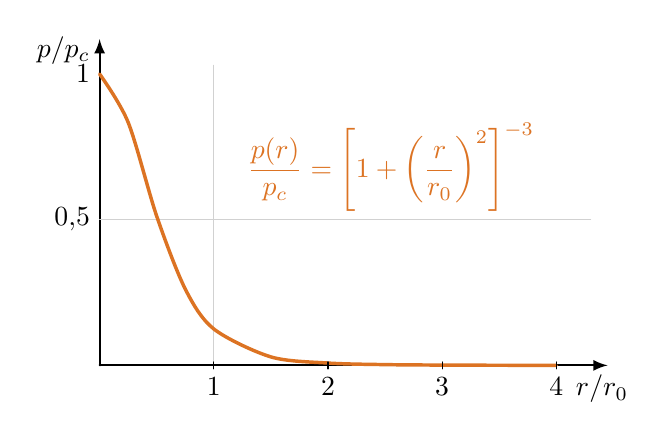
\begin{tikzpicture}[x=1.45cm,y=3.7cm,line cap=round,line join=round]
        \draw[-latex,line width=0.8pt] (0,0) -- (4.45,0);
        \draw[-latex,line width=0.8pt] (0,0) -- (0,1.12);
        \draw[black!18] (1,0) -- (1,1.03);
        \draw[black!18] (0,0.5) -- (4.30,0.5);

        \draw[pressureorange,line width=1.25pt,smooth]
            plot coordinates {
                (0,1) (0.25,0.834) (0.5,0.512) (0.75,0.262)
                (1,0.125) (1.5,0.0291) (2,0.008)
                (2.5,0.00262) (3,0.001) (3.5,0.00043) (4,0.00020)
            };

        \node[below] at (4.40,0) {$r/r_0$};
        \node[left] at (0,1.08) {$p/p_c$};
        \node[pressureorange,align=left] at (2.55,0.68)
            {$\displaystyle \frac{p(r)}{p_c}
            =\left[1+\left(\frac{r}{r_0}\right)^2\right]^{-3}$};

        \foreach \x in {1,2,3,4} {
            \draw (\x,0.012) -- (\x,-0.012);
            \node[below] at (\x,-0.01) {$\x$};
        }
        \node[left] at (0,0.5) {$0{,}5$};
        \node[left] at (0,1) {$1$};
    \end{tikzpicture}
    \caption{Perfil normalizado de presión obtenido en la parte (b) del problema 6.}
\end{figure}
